% !TeX spellcheck = en_US

\chapter{Image Segmentation with Convolutional Neural Networks (CNN)}\label{chp:segmentation_with_neural_networks}
\section{Introduction}
With the increasing computational power of recent graphic cards, increasingly complex neural networks can be used for increasingly challenging tasks. In the area of image processing, deep learning is gaining in popularity, partly because of the wide availability of data sets. In addition, companies recognize the vast amount of knowledge and information that can be retrieved with such technologies. The following sections provide a brief introduction to image segmentation using convolutional neural networks.

\section{Object detection and segmentation}
Object detection existed long before deep learning became popular. In object detection, the goal is to determine whether an object of a specified class (for example “car”) occurs within an image. Another type of object detection is additional classification, which means finding all objects in an image, together with their class, and calculating the probability that the object belongs to the determined class. \autoref{fig:neural_networks:object_detection} shows an example of object detection and classification.

\begin{figure}[H]
    \centering
	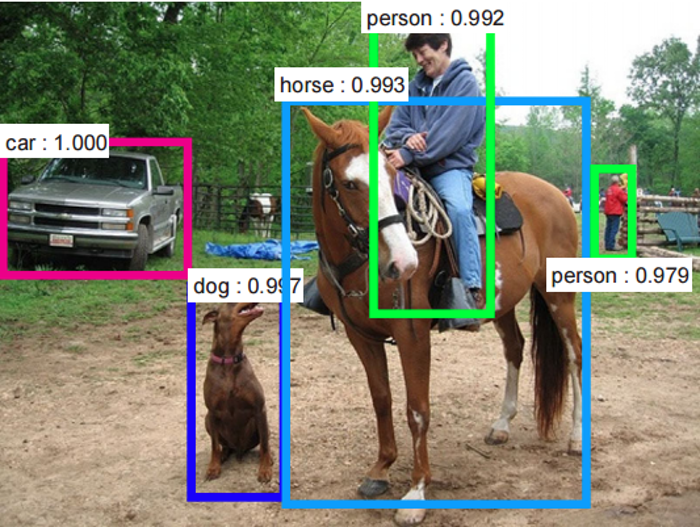
\includegraphics[width=0.6\linewidth]{chapters/neural_networks/images/object_detection.png}
	\caption{An example of object detection, showing the detected classes and the confidence level for each prediction.\\ Source: https://dius.com.au/2016/12/06/the-cleverness-of-deep-learning/ (27.05.2018)}
	\label{fig:neural_networks:object_detection}
\end{figure}

In contrast to object detection, the aim of image segmentation is not only to state whether an object occurs in the image but also to label each pixel of the image with a class, such as “car” or “building”. Different types of image segmentation are shown in \autoref{fig:neural_networks:image_segmentation}.

\begin{figure}[H]
    \centering
	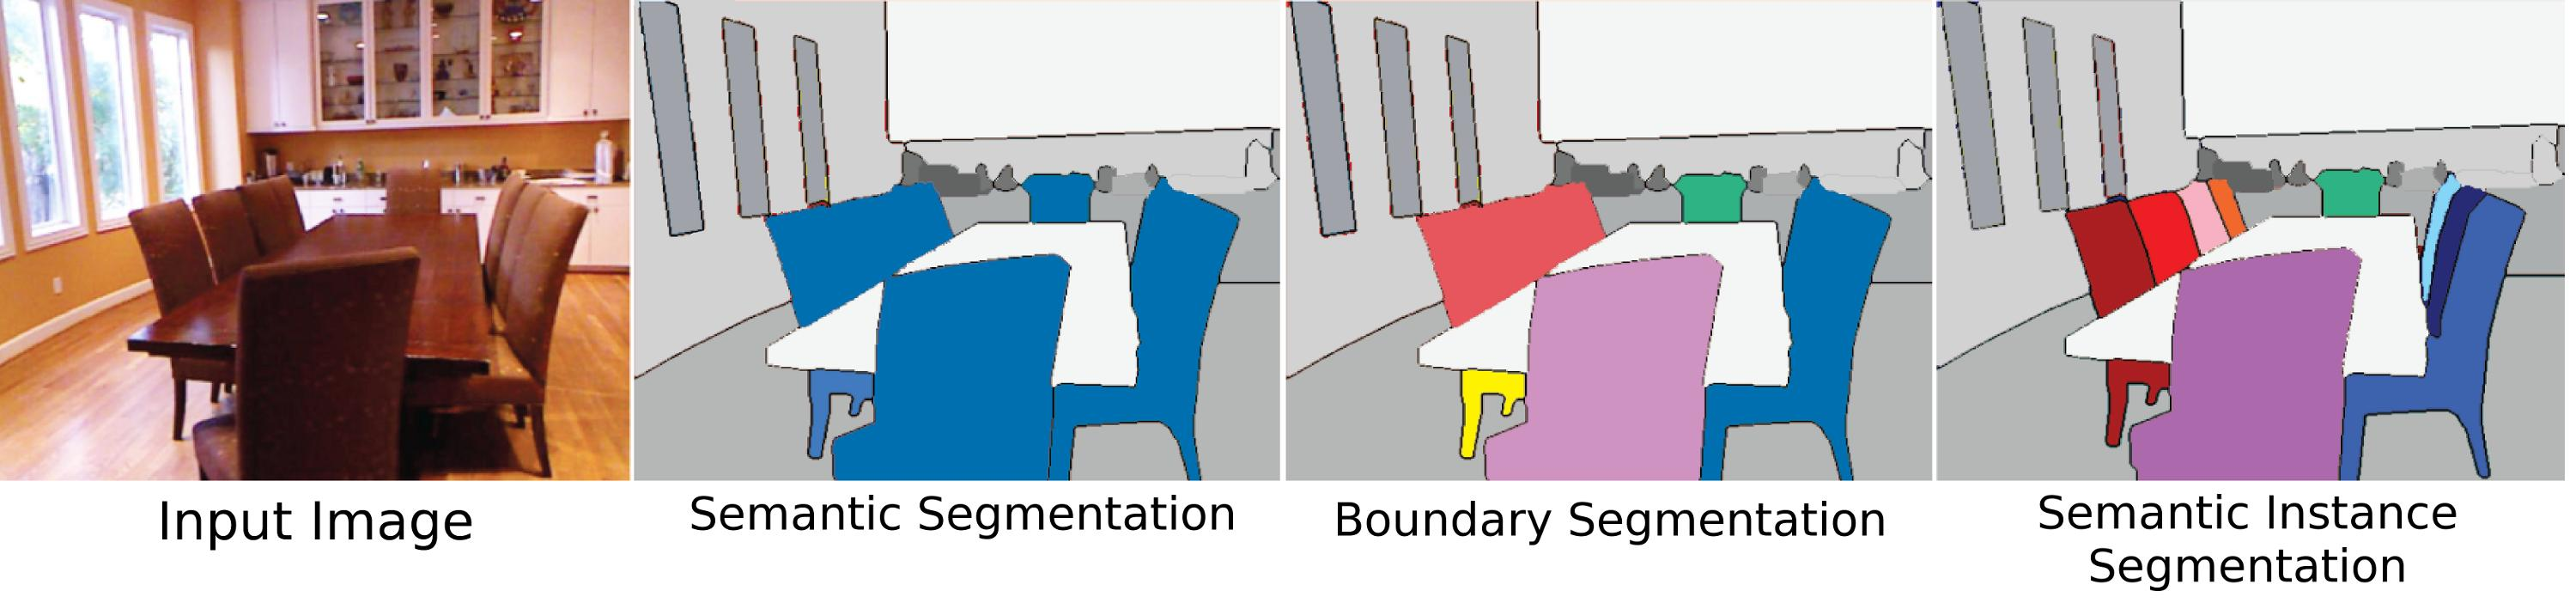
\includegraphics[width=0.8\linewidth]{chapters/neural_networks/images/segmentation.jpg}
	\caption{Types of image segmentation.\\ Source: https://i.stack.imgur.com/mPFUo.jpg (27.05.2018)}
	\label{fig:neural_networks:image_segmentation}
\end{figure}

\section{Convolutional Layer}
A convolutional layer is one of the most basic and important building blocks of a neural network. It has several filters, each of which is small compared to the input volume (the image) – for example, 5x5x3 pixels (a 5x5 filter with 3 channels, because standard images have 3 color channels). During the forward pass of the network, the filters are moved over the input image. At each position of the filters on the image, a convolution is computed, which is an element-wise matrix multiplication and a sum over the resulting matrix. The result of this operation is an activation map; this map is the output of the convolutional layer.

\begin{figure}[H]
    \centering
	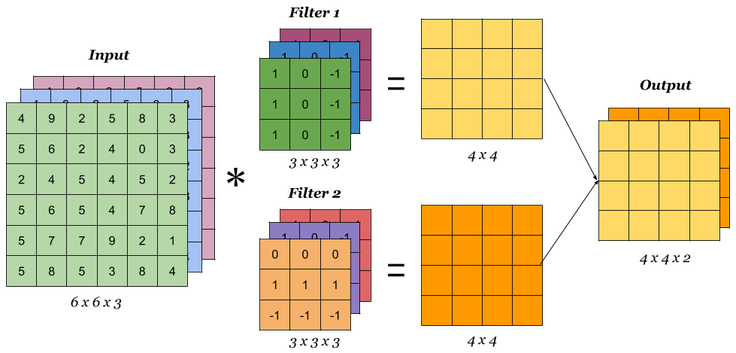
\includegraphics[width=0.8\linewidth]{chapters/neural_networks/images/convolution-with-multiple-filters.png}
	\caption{Convolution with multiple filters\\ Source: https://idoml.com (03.06.2018)}
	\label{fig:neural_networks:convolution_with_multiple_filters}
\end{figure}

The size of a filter can be configured, as well as the step size, the stride, and the amount of zero padding around the input image.

\begin{figure}[H]
    \centering
	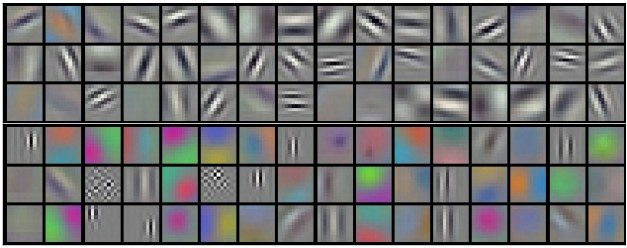
\includegraphics[width=0.6\linewidth]{chapters/neural_networks/images/example_filters.jpeg}
	\caption{Example filters learned by AlexNet \cite{Krizhevsky.2012}.\\ Source: http://cs231n.github.io/assets/cnn/weights.jpeg (27.05.2018)}
	\label{fig:neural_networks:example_filters}
\end{figure}

\section{Pooling Layer}
Pooling is a technique which allows reduction in the size of an image by extracting a single value from a region of values. The extracted value depends on the pooling type that is used. The most common pooling types are maximum (max) pooling for extracting the highest value from the current field, and average (avg) pooling, which extracts the average value of the current region.

A pooling layer has basically three parameters it can be configured with. First, there is the stride \textit{s}, which is the distance the filter is moved. Second, there is the filter size \textit{f}, which determines the width and height of the filter that is used to extract the value from the input.

\begin{figure}[H]
    \centering
	\begin{subfigure}{0.4\textwidth}
    	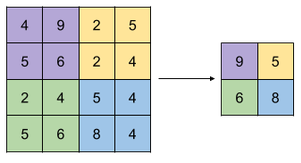
\includegraphics[width=0.9\linewidth]{chapters/neural_networks/images/max_pooling.png}		    \caption{Max Pooling}
    	\label{fig:neural_networks:max_pooling}
	\end{subfigure}~
	\begin{subfigure}{0.4\textwidth}
    	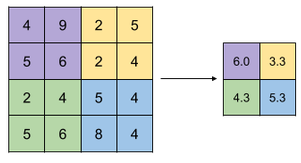
\includegraphics[width=0.9\linewidth]{chapters/neural_networks/images/avg_pooling.png}       	\caption{Average Pooling}
    	\label{fig:neural_networks:avg_pooling}
	\end{subfigure}
	\caption{Max and average pooling\\Source: https://idoml.com (02.06.2018)}
	\label{fig:neural_networks:pooling}
\end{figure}

As described in the previous chapter, a layer can have many output channels. Pooling can also be performed with multiple channels, as shown in \autoref{fig:neural_networks:max_pooling_multichannel}.

\begin{figure}[H]
    \centering
	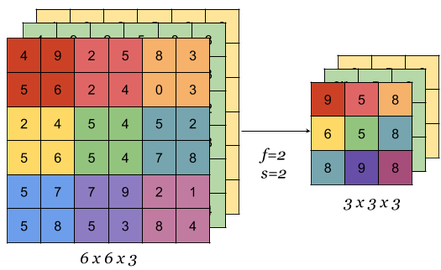
\includegraphics[width=0.6\linewidth]{chapters/neural_networks/images/max_pooling_multichannel.png}
	\caption{Max pooling with multiple channels\\ Source:https://idoml.com (03.06.2018)}
	\label{fig:neural_networks:max_pooling_multichannel}
\end{figure}

\section{Fully Connected Layer}
A fully connected layer is almost identical to a convolutional layer. The only difference is that the output of a convolutional layer is spatially connected to a region of the previous layer, but not to the whole output. \autoref{fig:neural_networks:fc_and_conv_layer} shows the difference between a fully connected layer and a convolutional layer.

\begin{figure}[H]
    \centering
	\begin{subfigure}{0.4\textwidth}
    	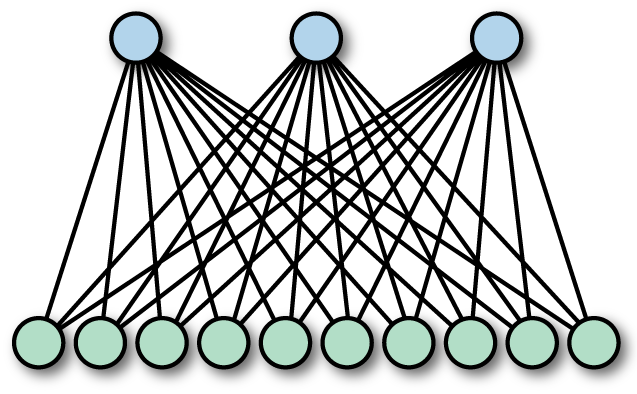
\includegraphics[width=0.9\linewidth]{chapters/neural_networks/images/fc_layer.png}		    \caption{Fully Connected Layer}
    	\label{fig:challenges:max_pooling}
	\end{subfigure}~
	\begin{subfigure}{0.4\textwidth}
    	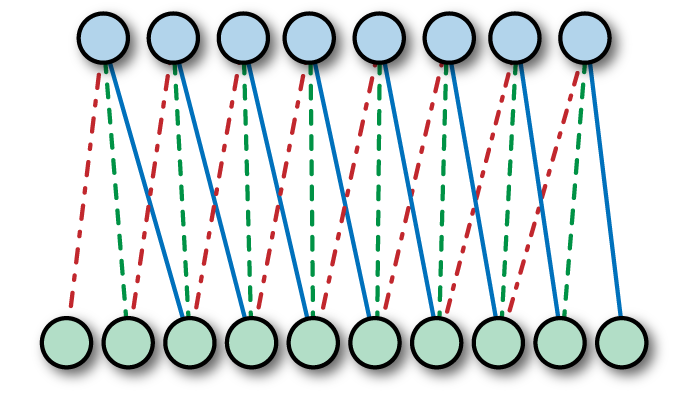
\includegraphics[width=0.9\linewidth]{chapters/neural_networks/images/conv_layer.png}       	\caption{Convolutional Layer}
    	\label{fig:challenges:avg_pooling}
	\end{subfigure}
	\caption{Fully Connected and Convolutional Layers\\Source: https://www.safaribooksonline.com/library/view/learning-tensorflow/9781491978504/ch04.html (07.06.2018)}
	\label{fig:neural_networks:fc_and_conv_layer}
\end{figure}

\section{Mask R-CNN}
A massive amount of research would be required to develop or improve an existing state-of-the-art neural network architecture. This was beyond the scope of the study, so we decided to use Mask R-CNN \cite{He.20170405}. As the name implies, this is a recurrent, convolutional neural network.